% A rebuild is deterministic: recompiling this recipe gives the same PDF, so
% hand-editing an output is pointless by construction.
% Every name on this figure is transcribed from the ten files frozen in
% ../intake/manifest.yaml. No number or name here is from memory.
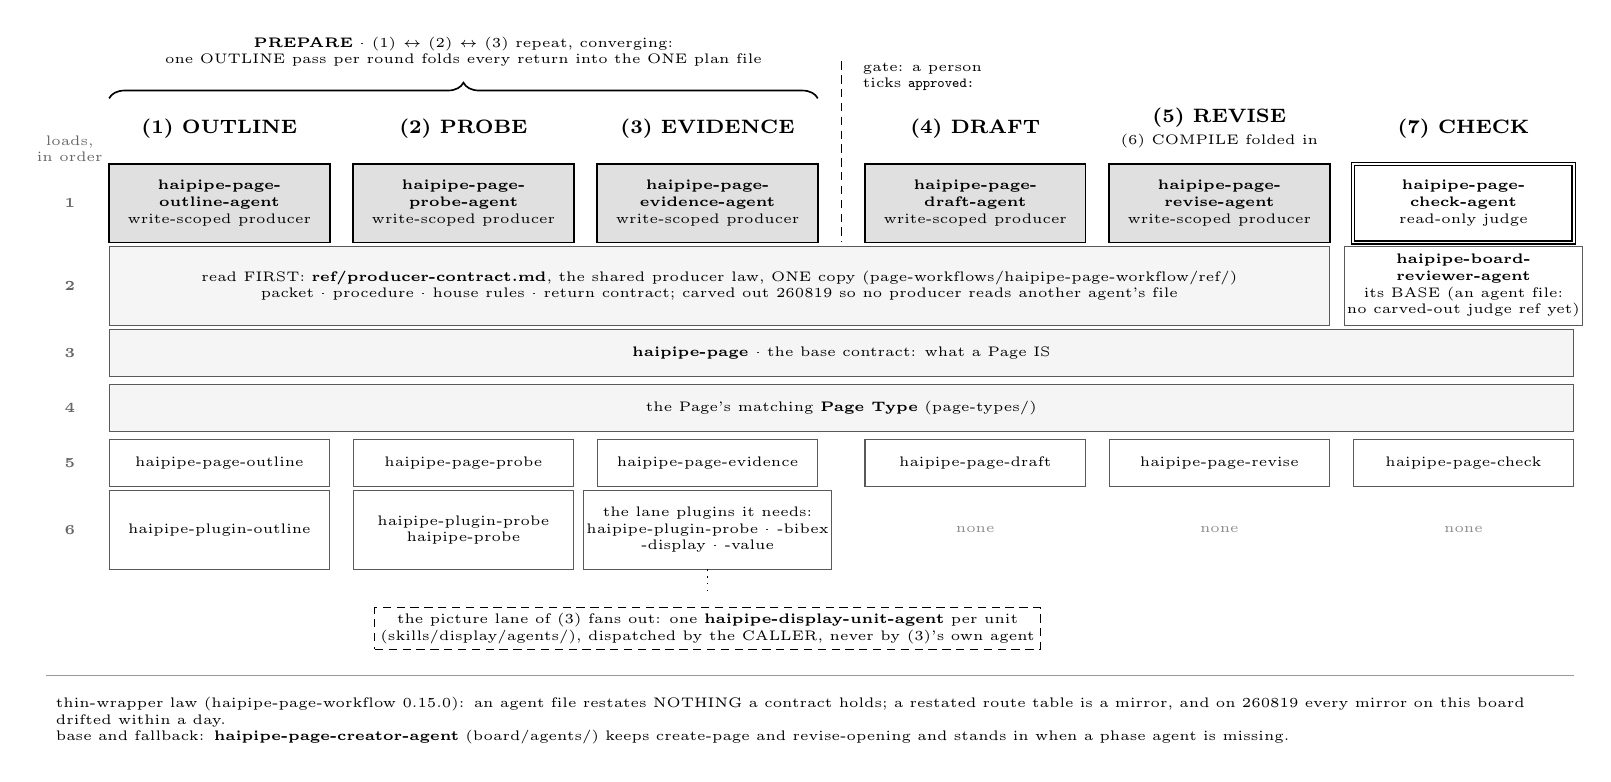
\begin{tikzpicture}[x=1mm, y=1mm,
  phasehead/.style={font=\scriptsize\bfseries, align=center, inner sep=1pt},
  agentbox/.style={draw, line width=0.7pt, fill=black!12, minimum width=28mm,
                   minimum height=10mm, font=\tiny, align=center, inner sep=1pt},
  judgebox/.style={draw, double, line width=0.5pt, fill=white, minimum width=28mm,
                   minimum height=10mm, font=\tiny, align=center, inner sep=1pt},
  cell/.style={draw, black!65, minimum width=28mm, minimum height=6mm,
               font=\tiny, align=center, inner sep=1pt, text=black},
  cellt/.style={cell, minimum height=10mm},
  spancell/.style={draw, black!65, fill=black!4, minimum height=6mm,
                   font=\tiny, align=center, inner sep=1pt, text=black},
  nonecell/.style={font=\tiny, text=black!45, align=center},
  loadnum/.style={font=\tiny\bfseries, text=black!60},
  note/.style={font=\tiny, align=center},
]

% ---- column centers: (1)(2)(3) then the gate, then (4)(5)(7) ----
% x: 0, 31, 62 | gate 79 | 96, 127, 158 · column width 28mm

% ---- the PREPARE bracket (this unit's one share of the iteration) ----
\draw[decorate, decoration={brace, amplitude=2mm}, line width=0.6pt]
  (-14,14.8) -- (76,14.8);
\node[note, anchor=south] at (31,17.6)
  {\textbf{PREPARE} · (1) $\leftrightarrow$ (2) $\leftrightarrow$ (3) repeat, converging:\\
   one OUTLINE pass per round folds every return into the ONE plan file};

% ---- the gate marker (the second share; routes stay Display4's) ----
\draw[densely dashed, line width=0.6pt] (79,19.5) -- (79,-3.5);
\node[font=\tiny, align=left, anchor=south west] at (80.5,14.5)
  {gate: a person\\ticks \texttt{approved:}};

% ---- phase headers, in the order the loop runs them ----
\node[phasehead] at (0,11)   {(1) OUTLINE};
\node[phasehead] at (31,11)  {(2) PROBE};
\node[phasehead] at (62,11)  {(3) EVIDENCE};
\node[phasehead] at (96,11)  {(4) DRAFT};
\node[phasehead] at (127,11) {(5) REVISE\\{\tiny\mdseries (6) COMPILE folded in}};
\node[phasehead] at (158,11) {(7) CHECK};

% ---- load order, down the left edge ----
\node[note, anchor=south, text=black!60] at (-19,5.5) {loads,\\in order};
\node[loadnum] at (-19,1.5)   {1};
\node[loadnum] at (-19,-9)    {2};
\node[loadnum] at (-19,-17.5) {3};
\node[loadnum] at (-19,-24.5) {4};
\node[loadnum] at (-19,-31.5) {5};
\node[loadnum] at (-19,-40)   {6};

% ---- row 1 · the executor, which IS its identity file ----
\node[agentbox] at (0,1.5)   {\textbf{haipipe-page-}\\\textbf{outline-agent}\\write-scoped producer};
\node[agentbox] at (31,1.5)  {\textbf{haipipe-page-}\\\textbf{probe-agent}\\write-scoped producer};
\node[agentbox] at (62,1.5)  {\textbf{haipipe-page-}\\\textbf{evidence-agent}\\write-scoped producer};
\node[agentbox] at (96,1.5)  {\textbf{haipipe-page-}\\\textbf{draft-agent}\\write-scoped producer};
\node[agentbox] at (127,1.5) {\textbf{haipipe-page-}\\\textbf{revise-agent}\\write-scoped producer};
\node[judgebox] at (158,1.5) {\textbf{haipipe-page-}\\\textbf{check-agent}\\read-only judge};

% ---- row 2 · the shared law, ONE copy; the judge rests on its base ----
\node[spancell, minimum width=155mm, minimum height=10mm] at (63.5,-9)
  {read FIRST: \textbf{ref/producer-contract.md}, the shared producer law, ONE copy
   (page-workflows/haipipe-page-workflow/ref/)\\
   packet · procedure · house rules · return contract; carved out 260819 so no
   producer reads another agent's file};
\node[cellt] at (158,-9)
  {\textbf{haipipe-board-}\\\textbf{reviewer-agent}\\its BASE (an agent file:\\no carved-out judge ref yet)};

% ---- rows 3 and 4 · shared by all six ----
\node[spancell, minimum width=186mm] at (79,-17.5)
  {\textbf{haipipe-page} · the base contract: what a Page IS};
\node[spancell, minimum width=186mm] at (79,-24.5)
  {the Page's matching \textbf{Page Type} (page-types/)};

% ---- row 5 · its own phase contract ----
\node[cell] at (0,-31.5)   {haipipe-page-outline};
\node[cell] at (31,-31.5)  {haipipe-page-probe};
\node[cell] at (62,-31.5)  {haipipe-page-evidence};
\node[cell] at (96,-31.5)  {haipipe-page-draft};
\node[cell] at (127,-31.5) {haipipe-page-revise};
\node[cell] at (158,-31.5) {haipipe-page-check};

% ---- row 6 · its plugins ----
\node[cellt] at (0,-40)  {haipipe-plugin-outline};
\node[cellt] at (31,-40) {haipipe-plugin-probe\\haipipe-probe};
\node[cellt] at (62,-40) {the lane plugins it needs:\\haipipe-plugin-probe · -bibex\\-display · -value};
\node[nonecell] at (96,-40)  {none};
\node[nonecell] at (127,-40) {none};
\node[nonecell] at (158,-40) {none};

% ---- the picture lane's fan-out, small ----
\draw[dotted, line width=0.5pt] (62,-45) -- (62,-48.5);
\node[note, draw, densely dashed, inner sep=2pt] at (62,-52.5)
  {the picture lane of (3) fans out: one \textbf{haipipe-display-unit-agent} per unit\\
   (skills/display/agents/), dispatched by the CALLER, never by (3)'s own agent};

% ---- the two laws under the roster ----
\draw[black!40, line width=0.4pt] (-22,-58.5) -- (172,-58.5);
\node[font=\tiny, align=left, text width=190mm, anchor=north west] at (-22,-60)
  {thin-wrapper law (haipipe-page-workflow 0.15.0): an agent file restates NOTHING
   a contract holds; a restated route table is a mirror, and on 260819 every mirror
   on this board drifted within a day.\\
   base and fallback: \textbf{haipipe-page-creator-agent} (board/agents/) keeps
   create-page and revise-opening and stands in when a phase agent is missing.};
\end{tikzpicture}
